\chapter{評価}
\label{evaluation}
\section{データ収集}
提案手法の有効性を確認するために,被験者9名(A$\sim$E,全員男性,平均年齢23歳)にプロトタイプデバイスを着用させ,サンプリングレート約30Hzでセンサデータを収集した.2秒間着用して取り外し,再び着用する試行を1セットとして被験者1人あたり計10セット(2秒$\times$20回分)を収集した.データ収集は1人当たり1 日最大4 セットとし,複数日に渡って実施した.センサと頭部のさまざまな位置関係のデータを収集するために,セット間に30 分以上の休憩時間を設けた.合計で2秒×10セット×9名=360秒のデータを収集した.今回の実験では1度の着用に対して1つのデータが必要なので,1回で収集した2秒間の平均値を解析に使用した.

\section{データ群の散らばり}
提案手法は距離に基づき装着者を識別する.すなわち,被験者ごとのデータ群に散らばりがなければ提案手法は成立しない.そのため,収集したすべてのデータに対して主成分分析を行い,2次元に圧縮したデータを2次元平面上にプロットし,目視で確認できるようにした.その結果を図\ref{PCA}に示す.\par

\begin{figure}[!t]
  \begin{center}
    \includegraphics[width=1\linewidth]{figure/PCA.eps}
  \end{center}
  \caption{PCAによる分析結果}
  \label{PCA}
\end{figure}

被験者A,Eのデータ群は分散が小さく,他の被験者のデータ群と重なりも見られない.被験者B,Iのデータ群は分散が小さいものの,互いに重なりが見られる.被験者Cのデータ群は分散が大きいが,1つのデータが被験者Iのデータ群に近い位置にあることを除き,他の被験者のデータ群との重なりは見られない.被験者D,Hのデータ群は分散が小さいが,互いにかなり重なっている.被験者F,Gのデータ群は分散が大きいものの,他の被験者のデータ群との重なりは見られない.\par
以上の結果は2次元に主成分分析しているため,データ量が大きく損失している.その点を考慮した上で,ヘルメット内部に搭載した圧力センサのデータから,距離に基づき装着者を識別できると判断した.

\section{提案手法での識別結果}
識別結果の評価指標として,FRR,FAR,EERを用いる.FRR(False reject rate:本人棄却率)は本人のデータを他人と誤って拒否してしまうことであり,FAR(False accept rate:他人受入率)とは他人のデータを本人と誤って認証してしまうことである.閾値を小さくするほどFRRが増加し,閾値を大きくするほどFARが増加する.これらはトレードオフの関係であり,FRRとFARが同値になるときの値をEER(Equal error rate:等価エラー率)と呼ぶ。このEERが小さいほど認証精度が良いとされる.\par
データセットに対し,被験者ごとに提案手法を用いて識別し評価指標を計算する.5分割交差検証を行って識別したときのFRRとFARの結果を図\ref{EER}に,EERの値を表\ref{EER_num}に示す.Totalは被験者全員の平均EERの値を示している.

\begin{figure}[H]
  \begin{center}
    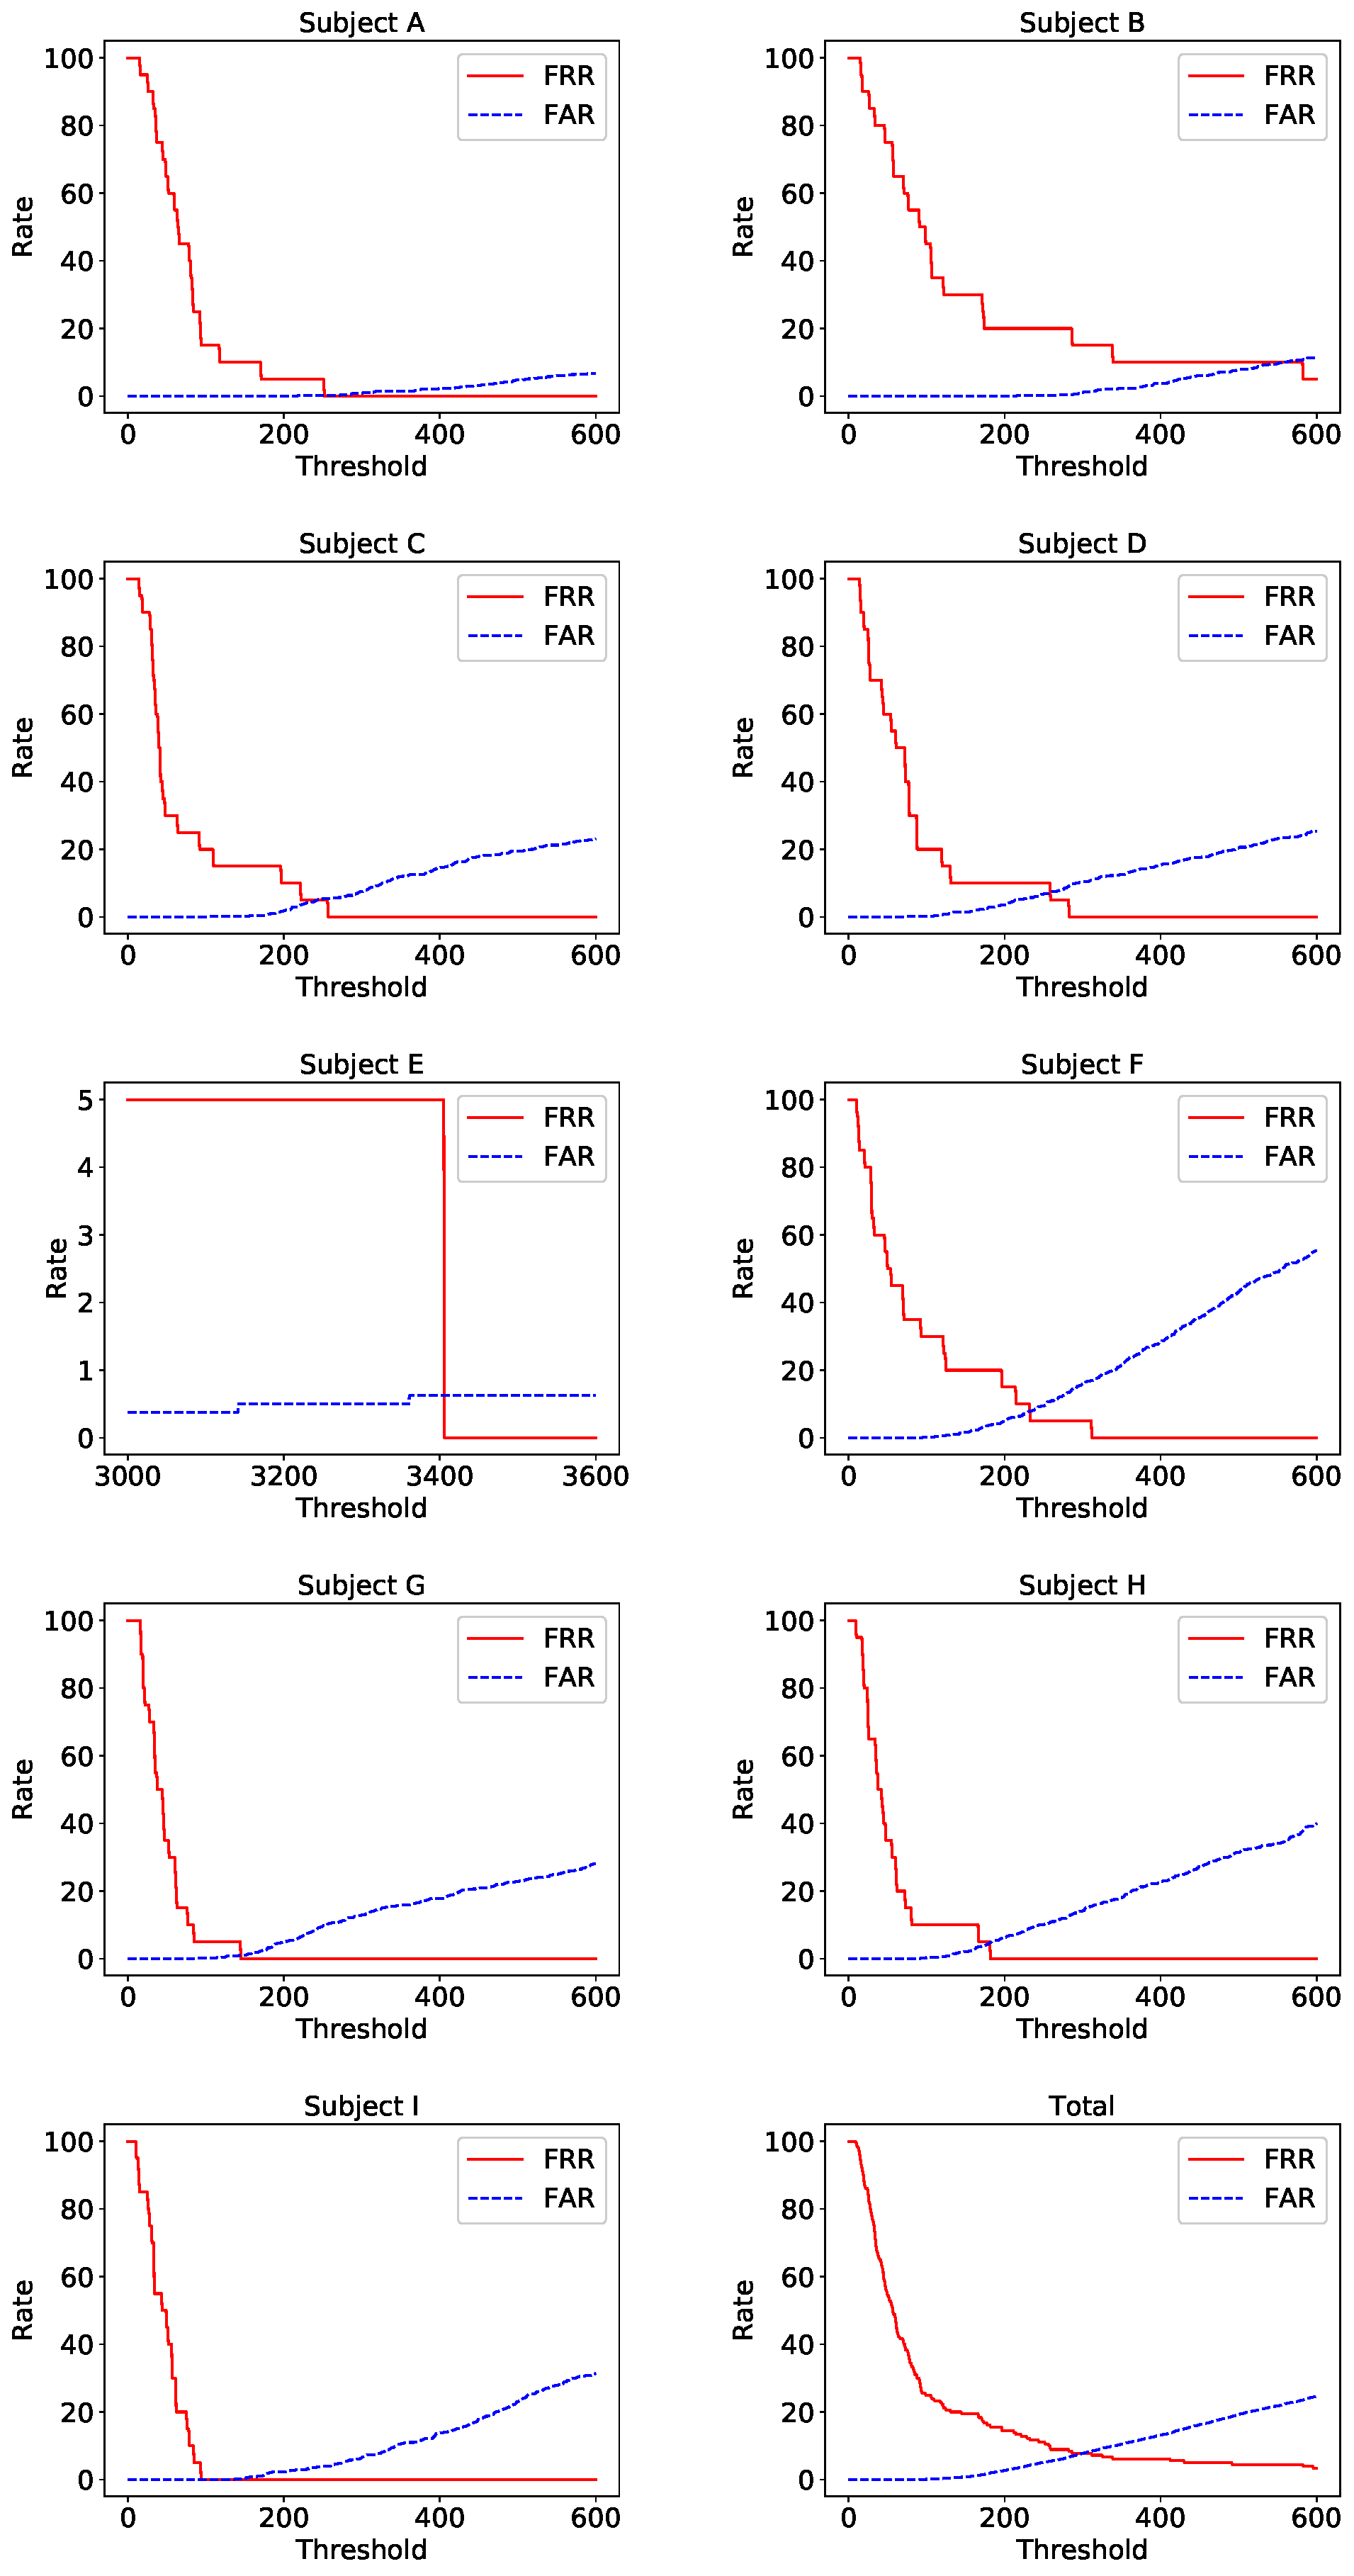
\includegraphics[height=1\textheight]{figure/EER.eps}
  \end{center}
  \caption{被験者ごとの判別結果}
  \label{EER}
\end{figure}

\begin{table}[htb]
  \centering
  \caption{被験者ごとのEER}
  \begin{tabular}{|c|c|} \hline
    被験者 & EER(\%) \\ \hline \hline
    A & 0.1 \\
    B & 10.0 \\
    C & 5.0 \\
    D & 7.3 \\
    E & 0.6 \\
    F & 7.9 \\
    G & 1.1 \\
    H & 4.6 \\
    I & 0.0 \\ \hline
    Total & 7.8 \\ \hline
  \end{tabular}
  \label{EER_num}
\end{table}

\section{識別結果の考察}
表\ref{EER_num}より被験者A,IのEERはほぼ0\%である.これは,検証に用いたデータセットでの識別が概ね完全にできたということを意味している.しかし,図\ref{PCA}では被験者Aと他の被験者のデータ群には重なりがなかったが,被験者Iは重なりが見られる.これは2次元に圧縮した際のデータの損失による影響だと考えられる.次いで結果が良かった被験者EのEERは約0.6\%だった.図\ref{PCA}より,被験者Eのデータ群はかなり隔離されていることが確認できる.しかし,図\ref{EER}を見ると,被験者EのみEERが得られた閾値が大きかったことがわかった.これも同様にデータの損失の影響であり,主成分分析で丸められているが生データでは外れ値が存在したため,FRRが下がりきる閾値が大きくなったと考えられる.他の被験者でも同様に,図\ref{PCA}のデータ群の重なりから予想されるEERと結果が異なる場合があったが,いずれもデータの損失による影響だと考えられる.また,被験者全員の平均EERは約7.8\%という結果であった.被験者ごとのEERに差が見られたことから,さらなる精度の向上を目指すことが可能であると考えられる.\par
提案手法ではマハラノビス距離を用いて識別を行うため,学習データ数をさらに増やすことで精度の向上が見込まれる.一方で,距離が同じ場合は識別が不可能となってしまう.その場合,提案手法と別の手法で識別を行う必要がある.具体的には,ヘルメットを装着する一連の流れを時系列データとして取得し,その特徴により識別を行う手法が考えられる.この手法が有効であるかを今後検証していく.